% Resultados e Discussão (versão compacta para o limite de 10 páginas). Versão completa: artigo/completo/resultados.tex.
% TODOS os números vêm de macros \N... (artigo/gerado/numeros.tex) e das tabelas de artigo/gerado/, geradas por
% `python -m analysis.artigo_numeros` a partir de outputs/analise/ e outputs/sensitivity_dora.csv, regenerados de
% data/metrics.csv (tag dataset-final). Não digitar números aqui. Conferência: `python -m analysis.artigo_numeros --check`.

\section{Resultados e Discussão}\label{sec:resultados}

Todas as análises partem de \texttt{data/metrics.csv} ($n = \NTotal$ repositórios) e reportam mediana e IQR,
com os cortes fixos da disciplina (Tabela~\ref{tab:resumo}). Release $\neq$ deploy e falha de CI $\neq$ falha em
produção; o CFR~(b) é \textbf{exploratório}, pois a heurística obteve F1 independente de 0,689, abaixo da meta de 0,70
(Seção~\ref{sec:heuristica}). A Tabela~\ref{tab:hipoteses} confronta as hipóteses da Introdução com os resultados.

\begin{table}[ht]
\centering\footnotesize
\caption{Mediana, quartis, IQR e classe DORA por métrica. ``Classe'' classifica a mediana; E/H/M/L são os
repositórios em Elite/High/Medium/Low. Recuperação: só repositórios com episódio concluído.}
\label{tab:resumo}
\resizebox{\linewidth}{!}{% Gerado por analysis/artigo_numeros.py a partir de outputs/analise/rq01_rq04_descritiva.csv. Não editar.
\begin{tabular}{llrrrrrll}
\hline
RQ & Métrica & $n$ & Mediana & Q1 & Q3 & IQR & Classe (mediana) & E/H/M/L \\ \hline
RQ01 & Deployment frequency (rel./sem.) & 300 & 0{,}36 & 0{,}19 & 0{,}77 & 0{,}58 & Medium & 6/55/143/96 \\
RQ02 & Lead time (a), por release (h) & 300 & 146{,}4 & 26{,}8 & 544{,}4 & 517{,}6 & High & 70/88/86/56 \\
RQ02 & Lead time (b), por commit (h) & 300 & 146{,}3 & 32{,}5 & 437{,}0 & 404{,}6 & High & 66/87/95/52 \\
RQ03 & CFR (a), proxy de CI (\%) & 300 & 5{,}7 & 2{,}4 & 14{,}1 & 11{,}7 & Elite & 229/40/17/14 \\
RQ03 & CFR (b), proxy de entrega (\%) & 299 & 20{,}0 & 4{,}1 & 46{,}5 & 42{,}4 & High & 121/67/33/78 \\
RQ04 & Recuperação (h) & 277 & 2{,}8 & 0{,}7 & 21{,}2 & 20{,}6 & High & 92/126/43/16 \\
\hline
\end{tabular}
}
\end{table}

\begin{table}[ht]
\centering\footnotesize
\caption{Hipóteses $\times$ resultados (expectativas na Introdução).}
\label{tab:hipoteses}
\begin{tabular}{@{}lp{11.2cm}l@{}}
\hline
\textbf{H} & \textbf{Observado (a expectativa está na Introdução)} & \textbf{Confirmada?} \\
\hline
H1 & Mediana \NDfMed{} rel./sem.; \NDfClasseHigh\% \textit{High} e \NDfClasseElite\% \textit{Elite} & Sim \\
H2 & Medianas iguais (\NLtaMed{} h e \NLtbMed{} h); por repositório, razão LT(a)/LT(b) com mediana \NRazMed{} (IQR \NRazQum--\NRazQtres) & Não \\
H3 & CFR(a) \NCfraMed\%; CFR(b) \NCfrbMed\% & Não \\
H4 & Mediana \NRecMed{} h; censurados: \NCensPct\% dos episódios & Parcial \\
H5 & CFR(a): $\rho = \NRhoA$; CFR(b): $\rho = \NRhoB$ & Parcial \\
H6 & \NSeisSig{} de \NSeisTestes{} testes significativos: idade (4), contribuidores (2), linguagem (2), efeito médio; tipo e popularidade, nenhum & Parcial \\
H7 & C1$\times$C2: \NSensUmDoisPct\%, $\kappa = \NSensUmDoisKappa$; C1$\times$C3: \NSensUmTresPct\%, $\kappa = \NSensUmTresKappa$ & Parcial \\
\hline
\end{tabular}
\end{table}

\begin{figure}[ht]
\centering
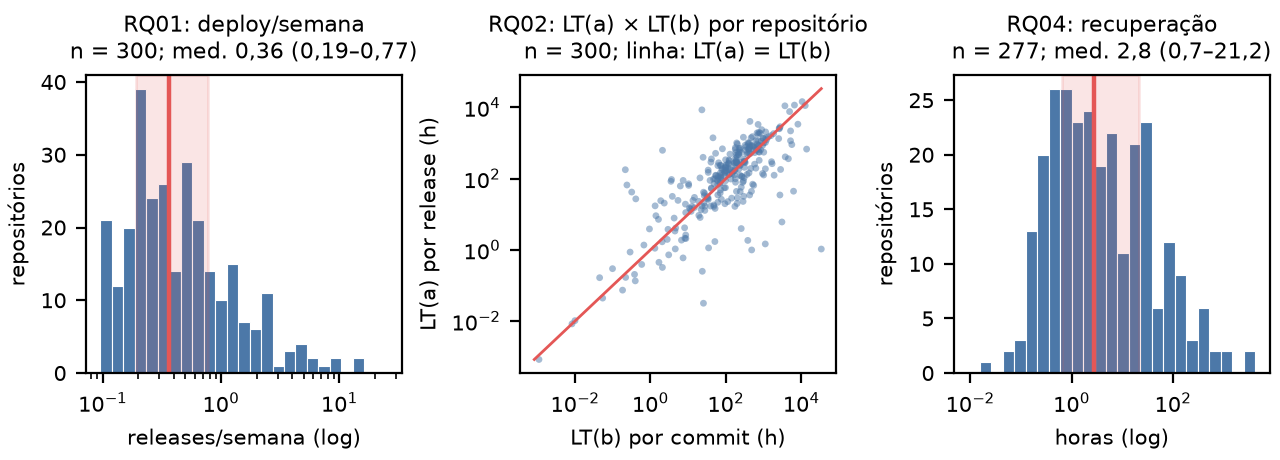
\includegraphics[width=\linewidth]{figs/fig_rq01_rq02_rq04.png}
\caption{RQ01, RQ02 e RQ04 por repositório (escala log). Linha e faixa vermelhas: mediana e IQR.}
\label{fig:rq124}
\end{figure}

\subsection{RQ01 --- Frequência de deploy}
A mediana foi de \textbf{\NDfMed{} releases/semana} (Q1 = \NDfQum; Q3 = \NDfQtres), pouco mais de uma \textit{release}
a cada três semanas, com cauda à direita (Figura~\ref{fig:rq124}). Pelos cortes da disciplina, \NDfClasseElite\%
são \textit{Elite}, \NDfClasseHigh\% \textit{High}, \NDfClasseMedium\% \textit{Medium} e \NDfClasseLow\% \textit{Low};
a classe geral C1 é \NUmClasseElite/\NUmClasseHigh/\NUmClasseMedium/\NUmClasseLow\% (E/H/M/L). A H1 se confirma.

\subsection{RQ02 --- Lead time for changes}
As medianas entre repositórios são \textbf{\NLtaMed{} h} para LT(a) ($\approx$ \NLtaDias{} dias; Q1 = \NLtaQum;
Q3 = \NLtaQtres) e \textbf{\NLtbMed{} h} para LT(b) (Q1 = \NLtbQum; Q3 = \NLtbQtres), ambas \textit{High}. Elas
coincidem, o que contraria a H2, mas só no agregado: por repositório a razão LT(a)/LT(b) tem mediana \NRazMed{} e
IQR \NRazQum--\NRazQtres; LT(a) supera o dobro de LT(b) em \NRazAdobroB\% dos repositórios, LT(b) supera o dobro de
LT(a) em \NRazBdobroA\% e só \NRazMeio\% ficam entre metade e o dobro (Wilcoxon pareado, $p$ \NRazWilcoxonP;
Figura~\ref{fig:rq124}). As variantes medem coisas diferentes: LT(a) usa o commit \emph{mais antigo} de cada
\textit{release}, e LT(b) pesa mais as \textit{releases} com muitos commits. Um commit antigo ``esquecido'' eleva
LT(a) sem mover muito LT(b), mas \NRazAmenorB\% dos repositórios têm LT(a) $<$ LT(b), o que ele não explica. Não
testamos causas: o lead time de cada commit está só no cache, não versionado.

\subsection{RQ03 --- Change failure rate}
O CFR~(a), proxy de CI, teve mediana de \textbf{\NCfraMed\%} (Q1 = \NCfraQum\%; Q3 = \NCfraQtres\%); o CFR~(b), proxy
de entrega, de \textbf{\NCfrbMed\%} (Q1 = \NCfrbQum\%; Q3 = \NCfrbQtres\%; $n = \NCfrbN$, pois um repositório tem menos
de duas \textit{releases} na janela). A H3 é refutada nos dois pontos. O CFR(a) conta \emph{execuções de CI} que
falharam, e falha de pipeline (teste instável, lint, ambiente) não é falha em produção; o CFR(b) conta
\textit{releases} seguidas de uma corretiva em 7 dias, segundo uma heurística imperfeita (F1 de 0,689), e mistura
correções reais com erros do proxy.

\subsection{RQ04 --- Tempo de recuperação}\label{sec:resultados-rq04}
A mediana foi de \textbf{\NRecMed{} h} (Q1 = \NRecQum; Q3 = \NRecQtres; $n = \NRecN$), classe \textit{High}.
\textbf{Censura:} \NCensEp{} de \NCensTot{} episódios (\NCensPct\%) não terminaram na janela; entre os \NCensReposCom{}
repositórios com episódio, a mediana da proporção de censurados é \NCensRepoMed\% (Q3 = \NCensRepoQtres\%) e
\NCensReposAlgum{} têm ao menos um censurado. Os censurados não entram na mediana, mas são contados. Dos
\NRecSemValor{} repositórios sem valor, \NCensReposSem{} não tiveram episódio e \NCensSoCens{} só tiveram censurados,
o que tende a subestimar a recuperação, pouco dado o volume de censura. A H4 se confirma só em parte: a mediana está
entre 1 h e 1 dia, mas a censura é bem menor que a esperada.

\begin{figure}[ht]
\centering
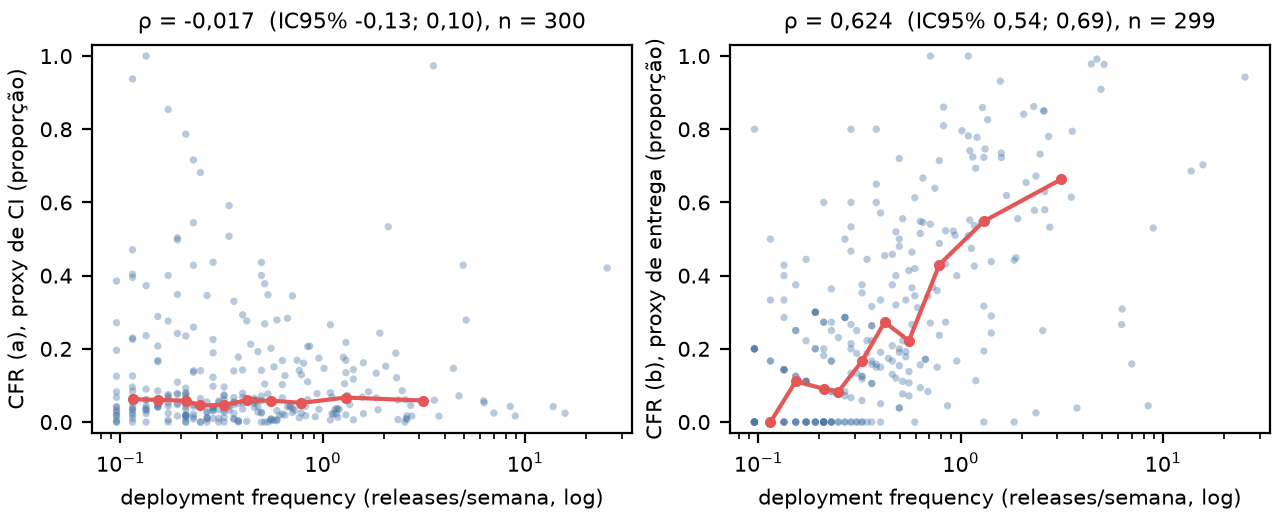
\includegraphics[width=\linewidth]{figs/fig_rq05.png}
\caption{RQ05: DF (escala log) $\times$ CFR(a) e CFR(b); linha vermelha: mediana do CFR por faixa de DF.}
\label{fig:rq05}
\end{figure}

\subsection{RQ05 --- Frequência de deploy $\times$ CFR}
Com o CFR(a), $\rho = \NRhoA$ ($p = $ \NRhoPA; IC 95\% \NRhoIcA; $n = \NRhoNA$): sem relação monotônica detectável.
Com o CFR(b), $\rho = \NRhoB$ ($p$ \NRhoPB; IC 95\% \NRhoIcB; $n = \NRhoNB$): correlação positiva forte
(Figura~\ref{fig:rq05}); os intervalos usam a transformação $z$ de Fisher com erro-padrão de Bonett e
Wright~\cite{bonett2000spearman}. A H5 se confirma só para (a). Isso não refuta a tese DORA, e correlação não implica
causalidade: o CFR(b) é acoplado mecanicamente à frequência (mais \textit{releases}, mais chances de uma corretiva em
7 dias), e com poucas \textit{releases} há muitos zeros. Com ao menos 20 \textit{releases} avaliadas, $\rho$ cai para
\NRhoBVinte{} ($n = \NRhoBVinteN$), mas isso também restringe a faixa de DF. A idade confunde (RQ06). O resultado (b) é um possível artefato, e o (a) é compatível com a tese.

\subsection{RQ06 --- Características dos repositórios}
Testamos cinco fatores (linguagem, popularidade, contribuidores, idade, tipo; $n = \NTipoN$ no tipo) contra as seis
métricas, \NSeisTestes{} testes. Todos os fatores têm três ou mais grupos, então todos usaram Kruskal-Wallis; Mann-Whitney
e o $\delta$ de Cliff~\cite{cliff1993dominance} (magnitude de Romano et al.~\cite{romano2006appropriate}) não foram
exercitados com dados reais, e o $\delta$ aparece só como contraste descritivo em \texttt{rq06\_testes.csv}. Os
p-valores foram corrigidos por Holm~\cite{holm1979sequentially} sobre os \NSeisTestes{} testes, e o efeito é
$\varepsilon^2 = H/(n-1)$, com a escala de Mangiafico~\cite{mangiafico2016handbook} (pequeno de $0{,}01$ a $<0{,}08$, médio até
$<0{,}26$; orientação do autor, não padrão; ``desprezível'' ($<0{,}01$) é rótulo nosso).
\textbf{\NSeisSig{} associações} permaneceram significativas, todas de efeito médio (Tabela~\ref{tab:rq06},
Figura~\ref{fig:rq06}). Os mais jovens (Q1 de idade) publicam mais (DF \NIdadeDfQum{} contra \NIdadeDfQquatro{}
rel./sem. no Q4), têm LT(a) menor (\NIdadeLtaQum{} h contra \NIdadeLtaQquatro{} h) e CFR(b) maior (\NIdadeCfrbQum\%
contra \NIdadeCfrbQquatro\%), em linha com o acoplamento da RQ05; mais contribuidores, LT(a) maior (\NContribLtaQum{} h
no Q1 contra \NContribLtaQquatro{} h no Q4); Rust tem os menores LT(a) e JavaScript a recuperação mais rápida. Popularidade (menor $p_{\mathrm{Holm}}$ = \NPopMinPHolm) e tipo não foram
significativos, e no tipo o $n$ limita o poder. A H6 é parcial: linguagem pesa mais que popularidade, mas o tipo não se
destaca, e idade e contribuidores têm efeito médio, não pequeno. São associações, não causas.

\begin{table}[ht]
\centering\footnotesize
\caption{RQ06: associações significativas após Holm (Kruskal-Wallis, $\varepsilon^2 = H/(n-1)$); os \NSeisTestes{} testes
estão em \texttt{outputs/analise/rq06\_testes.csv}.}
\label{tab:rq06}
\resizebox{\linewidth}{!}{% Gerado por analysis/artigo_numeros.py a partir de outputs/analise/rq06_testes.csv. Não editar.
\begin{tabular}{llrrrrl}
\hline
Fator & Métrica & $n$ & $H$ & $p_{\mathrm{Holm}}$ & $\varepsilon^2$ & Magnitude \\ \hline
Idade & Lead time (a) por release & 300 & 64{,}8 & $<0{,}001$ & 0{,}217 & médio \\
Idade & Lead time (b) por commit & 300 & 51{,}2 & $<0{,}001$ & 0{,}171 & médio \\
Idade & CFR (b) proxy de entrega & 299 & 40{,}3 & $<0{,}001$ & 0{,}135 & médio \\
Idade & Deployment frequency & 300 & 36{,}2 & $<0{,}001$ & 0{,}121 & médio \\
Contribuidores & Lead time (a) por release & 300 & 33{,}8 & $<0{,}001$ & 0{,}113 & médio \\
Contribuidores & Lead time (b) por commit & 300 & 26{,}0 & $<0{,}001$ & 0{,}087 & médio \\
Linguagem & Lead time (a) por release & 298 & 24{,}9 & $0{{,}}0087$ & 0{,}084 & médio \\
Linguagem & Tempo de recuperação & 276 & 22{,}2 & $0{{,}}025$ & 0{,}081 & médio \\
\hline
\end{tabular}
}
\end{table}

\begin{figure}[ht]
\centering
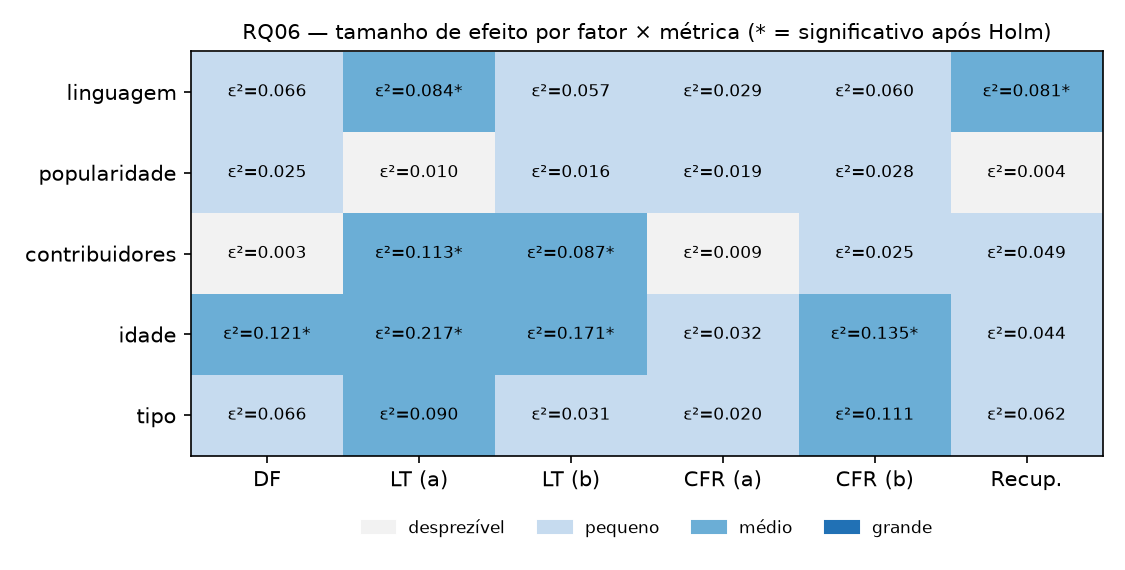
\includegraphics[width=.66\linewidth]{figs/rq06_efeitos.png}
\caption{RQ06: $\varepsilon^2$ por fator e métrica (* = significativo após Holm).}
\label{fig:rq06}
\end{figure}

\subsection{RQ07 --- Sensibilidade das classificações}
Comparamos C1 (release, LT(a), CFR(a)), C2 (release e pré-release, LT(b), CFR(b)) e C3 (tag, LT(b), CFR(a)), com
categorias codificadas de 1 a 4 e $\kappa$ linear ponderado~\cite{cohen1968weighted} (Figura~\ref{fig:rq07}).
C1$\times$C2 muda em \NSensUmDoisPct\% dos repositórios ($\kappa = \NSensUmDoisKappa$, moderado), o que confirma
a H7; C1$\times$C3 em \NSensUmTresPct\% ($\kappa = \NSensUmTresKappa$) e C2$\times$C3 em \NSensDoisTresPct\%
($\kappa = \NSensDoisTresKappa$), ambos substanciais, abaixo de 30\%. \textbf{Limitações:} em C2 e C3 só a unidade do DF
muda (LT(b) e CFR(b) seguem sobre releases), e \NParcialCUm, \NParcialCDois{} e \NParcialCTres{} repositórios em C1, C2 e C3
são classificados com três métricas.

\begin{figure}[ht]
\centering
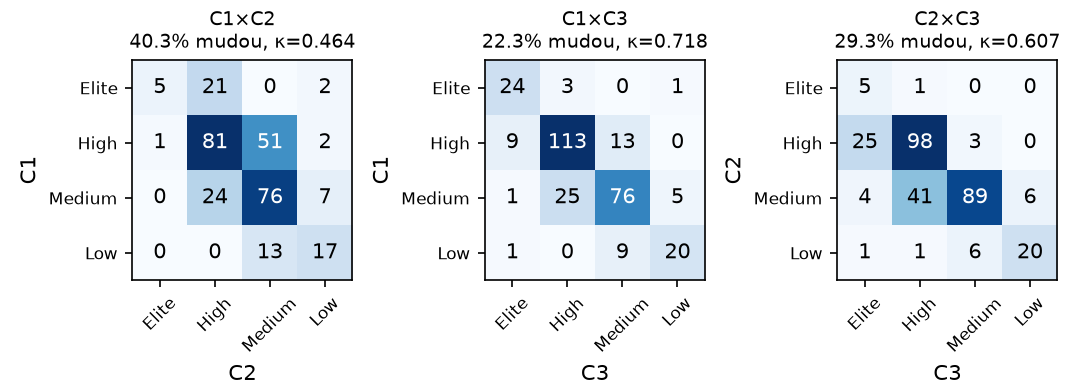
\includegraphics[width=.92\linewidth]{figs/sensitivity_transicao.png}
\caption{RQ07: matrizes de transição entre combinações (linha = primeira; coluna = segunda).}
\label{fig:rq07}
\end{figure}

\textbf{Robustez de RQ01--RQ06.} A maior discordância é C1$\times$C2, que troca CFR(a) por CFR(b) além da unidade de
deploy, coerente com as RQ03 e RQ05: as conclusões sobre CFR dependem da definição, e a de DF$\times$CFR(b) é a menos
robusta. As associações de LT da RQ06 aparecem em LT(a) e LT(b). A RQ01 depende da unidade de deploy (em C1$\times$C3,
\NSensUmTresPct\% mudam de classe), e a RQ04 não tem variante. Na análise ampliada, só quatro das sete variações
reclassificam de fato (janela do CFR(b) e cortes $\pm 10\%$): mudam \NAmpInfMinPct\% a \NAmpInfMaxPct\% dos repositórios,
com $\kappa \geq \NAmpInfKappaMin$; as outras três dão 0\% por construção e não são evidência de robustez. A classificação
é estável a pequenas perturbações dos cortes, mas depende da unidade de deploy e da variante de CFR.

\subsection{RQ08 --- Rework rate (bônus)}
A \textit{rework rate} (proporção de \textit{releases} corretivas) teve mediana de \textbf{\NRwMed\%} (Q1 = \NRwQum\%;
Q3 = \NRwQtres\%; $n = \NRwN$), contra \NRwCfrbMed\% do CFR(b) no subconjunto pareado. Três repositórios ficam fora (dois sem
rótulos no cache, um com contadores divergentes do \texttt{metrics.csv}). A diferença pareada
tem mediana 0, mas IQR de \NRwDifIqr{} p.p. e Wilcoxon $p = $ \NRwWilcoxonP; $\rho = \NRwSpearman$ entre as duas. As medidas
não são equivalentes: o CFR(b) conta a \textit{release} que \emph{precisou} de correção, e o rework a que \emph{é}
correção. Ambas herdam a imprecisão da heurística v12.
